\documentclass[10pt,a4paper]{article}
\usepackage[utf8]{inputenc}
\usepackage{amsmath}
\usepackage{amsfonts}
\usepackage{amssymb}
\usepackage{siunitx}
\usepackage{booktabs}
\usepackage{hyperref}
\usepackage{graphicx}
\usepackage{mathrsfs}
\graphicspath{{../figures/}}
\usepackage{subfig}
\newcommand{\kev}{\si{\kilo\electronvolt}}
\newcommand{\mev}{\si{\mega\electronvolt}}
\newcommand{\gev}{\si{\giga\electronvolt}}
\title{FYS4505 - Assignment 1: Radiation-matter interaction}
\author{Federico Nardi}
\date{\vspace{-5ex}}
\begin{document}
\maketitle

% -----------------------------------------------------------

\section*{Problem 1: Stopping power}

\begin{enumerate}

\item[a)] First of all we need to get the relativistic parameters $\beta^2$ and $\gamma$. The latter can be easily found by inverting the relation
\begin{align*}
E_{beam} = \tau = (\gamma - 1 )\,M c^2
\end{align*}
where $M$ is the mass of the beam particles. We can get the other parameter by inverting the definition of $\gamma$:
\begin{align*}
\beta^2 = 1 - \frac{1}{\gamma^2}.
\end{align*} 
The source for absorber material parameters of density $\rho$ and mean excitation energy $I$ is the US National Institute of Standards and Technology (NIST)\footnote{\url{https://physics.nist.gov/cgi-bin/Star/compos.pl?matno=014}} while for atomic numbers $Z$ and mass numbers $A$ an usual periodic table has been used. Table \ref{tab:absorbers} provides a summary of those parameters.
\begin{table}[!ht]
\centering
\begin{tabular}{ccccc}
\toprule
  & $\rho\,[\si{\gram\per\cubic\centi\meter}]$ & $I\,[\si{\electronvolt}]$ & $Z$ & $A$ \\
  \midrule
  Si & $2.33$ & $173.0$ & $14$ & $28.085$\\
  Ge & $5.323$ & $350.0$ & $32$ & $72.63$ \\
  \bottomrule
\end{tabular}
\caption{Physical parameters of absorber materials}
\label{tab:absorbers}
\end{table}
The incoming beam is made of $\alpha$-particles, $^4_2$He nuclei with $M=3.727\si{\giga\electronvolt}$ and $z=2$. 
All those parameters have been inserted in a Python code implementing the Bethe-Bloch formula \footnote{\url{https://github.com/FedericoNardi/Instrumentation-Task1}}, giving the results in Table \ref{tab:alphabeam}.\
\begin{table}[!ht]
\centering
\begin{tabular}{ccc}
\toprule
  & $\S\,[\si{\mega\electronvolt\per\centi\meter}]$ & $\frac{S}{\rho}\,[\si{\mega\electronvolt\gram\per\square\centi\meter}]$\\
  \midrule
  Si & $1470.02$ & $630.91$ \\
  Ge & $2210.75$ & $415.32$\\
  \bottomrule
\end{tabular}
\caption{Stopping power for alpha particle beam in Silicon and Germanium}
\label{tab:alphabeam}
\end{table}

The value $\frac{S}{\rho}$ has been used as a test to compare the results with figure 2.4 in \cite{Tavernier}, predicting a stopping power of about $600\si{\mega\electronvolt\gram\per\square\centi\meter}\si{\mega\electronvolt\gram\per\square\centi\meter}$ and $400\si{\mega\electronvolt\gram\per\square\centi\meter}$ respecively for a $5\si{\mega\electronvolt}$ alpha particle beam.

\item[b)] When the incoming beam is made of electrons, the Bethe-Bloch formula needs to be modified in order to consider the electron-electron interactions, including spin interactions and Pauli repulsion between identical fermions. 
The value of $T_{max}$ for maximum energy transfer to electron is replaced by the kinetic energy $\frac{\tau}{2}$ of the incoming electrons and we have an additional correction term $F(\tau)$ defined as
\begin{align*}
F(\tau) = 1-\beta^2 + \frac{ \frac{\tau^2}{8} - (2\tau+1)\log(2) }{(\tau+1)^2}
\end{align*}

\item[c)] The corrections discussed in b) have been implemented in the code used in a) with an if selection on a flag for electrons. The results are shown in Table \ref{tab:electronbeam}.
\begin{table}[!ht]
\centering
\begin{tabular}{cc}
\toprule
  & $\S\,[\si{\mega\electronvolt\per\centi\meter}]$ \\
  \midrule
  Si & $3.88$ \\
  Ge & $7.33$ \\
  \bottomrule
\end{tabular}
\caption{Stopping power for alpha particle beam in Silicon and Germanium}
\label{tab:electronbeam}
\end{table}
As expected, the penetrating power of electrons is much higher with respect to alpha particles, and the energy lost through the material is almost three order of magnitude smaller. This is due mostly to the smaller size of electrons, that reduces the number of collisions in the material increasing the mean free path of the particles. 
\end{enumerate}

%-----------------------------------------

\section*{Problem 2: Shielding calculation}
\begin{enumerate}

\item[a)] First, we compare the stopping power obtained by applying Bragg rule and the one computed with empirical values for Portland concrete from NIST in the energy range we are interested in. The results, displayed in figure \ref{fig:Bragg}, differ in the best case by at least a factor 2 and therefore the value for mean excitation energy cannot be explained just as a sum of weighted contributions. 

\begin{figure}
\centering
\subfloat[]{
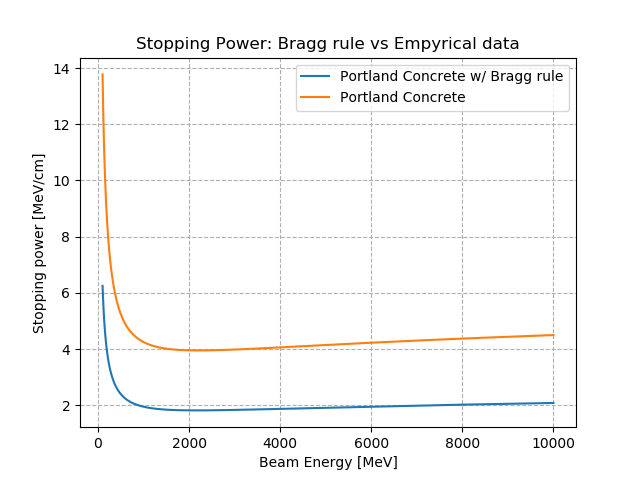
\includegraphics[width=0.6\textwidth]{Bragg.png}\label{fig:Bragg}
}
\subfloat[]{
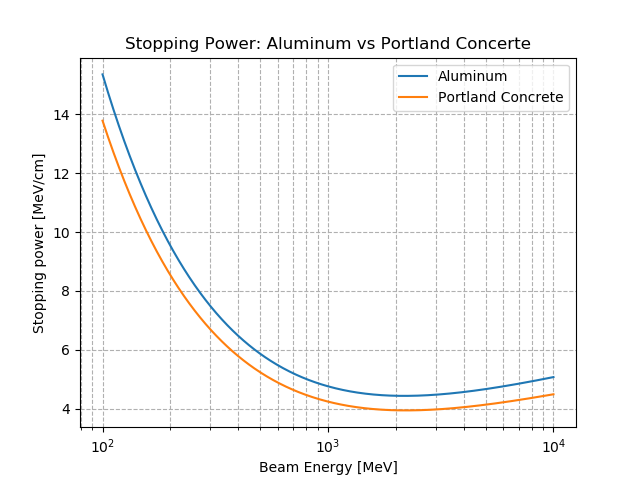
\includegraphics[width=0.6\textwidth]{AlvsPC.png}
\label{fig:versus}
}
\caption{Stopping power from Bragg rule and from empirical data for Portland Concrete (a) and comparison between Aluminum and Portland Concrete stopping power (b).}
\end{figure}

When compared with aluminum (figure \ref{fig:versus}) the stopping power of concrete is never more than $2\si{\mega\electronvolt\per\centi\meter}(20\si{\percent})$ higher than the one of aluminum in our energy range,  meaning that we would need a $20\%$ thicker block of concrete to have for the same performance as an aluminum block. If we consider the same volume of material, the ratio between the cost of the materials is \footnote{For portland concrete, assuming we won't need to buy tons of it: \url{https://www.alibaba.com/showroom/portland-cement-prices.html}, while for aluminum: \url{https://markets.businessinsider.com/commodities/aluminum-price}}
\begin{align*}
\frac{\rho[Concrete]}{\rho[Al]}\times\frac{0.2\,\$\,\si{\per\kilo\gram}}{2.07\,\$\,\si{\per\kilo\gram}}\sim 10
\end{align*}
meaning that aluminum would cost 10 times more only to have a $20\si{\percent}$ better performance. Therefore for budget purposes, assuming that the code works properly and the stopping power values are correct, we should choose Portland concrete. 
However for the rest of the exercise will be considered Aluminum, since it's easier to compare the results with literature and being a single element we don't need to average on more values.

\item[b)] Further corrections to the Bethe formula can include a shell correction and a density correction term
\begin{itemize}
\item The shell correction becomes relevant for beam energies comparable to orbital elecron momenta, i.e. under $\sim1\si{\kilo\electronvolt}$, where we cannot assume anymore that the electrons are at rest with respect to the beam particles. That is not our case, since the minimum energy for our protons is much higher - at least $5$ orders of magnitude.
\item the density correction term is due to a local polarization due to the field of the incoming particle resulting in a shielding effect on the outer electrons, that will contribute with less collisions to the energy loss.
We therefore need to subtract a term $\delta$ to the logarithmic behaviour of Bethe-Bloch formula. The code uses the expression from \cite{Leo}. The result is shown in figure \ref{fig:BetheCorrected}.\\
First, at lower energies, when increasing the beam velocity the collisions between beam particles and electrons in the material are less and less frequent and the stopping power drops. It reaches a minimum before increasing again: here the energies are high enough that, despite the fewer collision, the momentum transfer in those events gives significant effects raising the stopping power. As expected, the density correction lowers the stopping power of the higher energy region because of the minor collision frequency induced by local polarization of the absorber. The minimum in the curves corresponds to the minimum ionization energy, marked in figure \ref{fig:BetheCorrected} with the two vertical lines, whose values are
\begin{align*}
\begin{split}
&\bar{E} = 2.18 \si{\giga\electronvolt}\qquad \text{without density correction}\\
&\bar{E} = 2.46 \si{\giga\electronvolt}\qquad \text{with density correction}
\end{split}
\end{align*}

\begin{figure}[!ht]
\centering
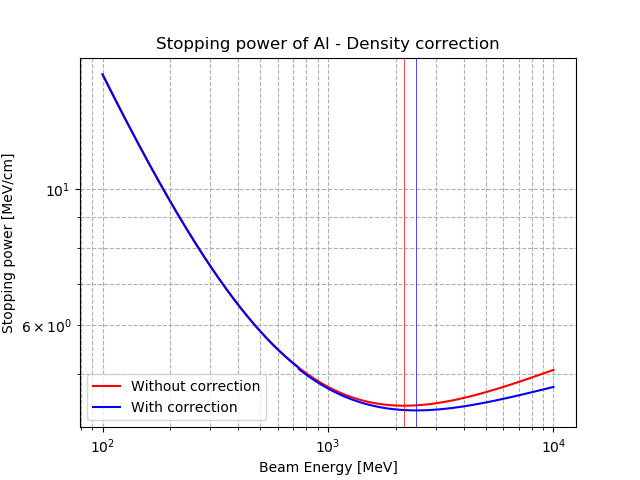
\includegraphics[width=0.7\textwidth]{BetheVsBethe++.png}
\caption{Stopping power of aluminum for protons with and without density correction term. The corresponding minimum ionization energies are marked with vertical lines with the same color of the corresponding curve.}
\label{fig:BetheCorrected}
\end{figure}

\item[c)] To get the range for a given material it is sufficient to integrate the Stopping Power $S(E)$ relation from Problem 1 with the minus sign (being an energy loss the gradient must be negative):
\begin{align*}
Range(E_{Beam}) = - \int_{E_{Beam}}^0\bigg( \frac{dE}{dx} \bigg)^{-1} dE = \int_{0}^{E_{Beam}}\frac{dE}{S(E)}
\end{align*}
The integration has been performed numerically for beam energies in the range of the problem, giving the results shown in figure \ref{fig:range}. 
Therefore, to stop a $10\si{\giga\electronvolt}$ proton, and therefore prevent all radiation to escape from our detector, the minimum thickness required is
\begin{align*}
d = 20.6\si{\metre}.
\end{align*}

\begin{figure}[!ht]
\centering
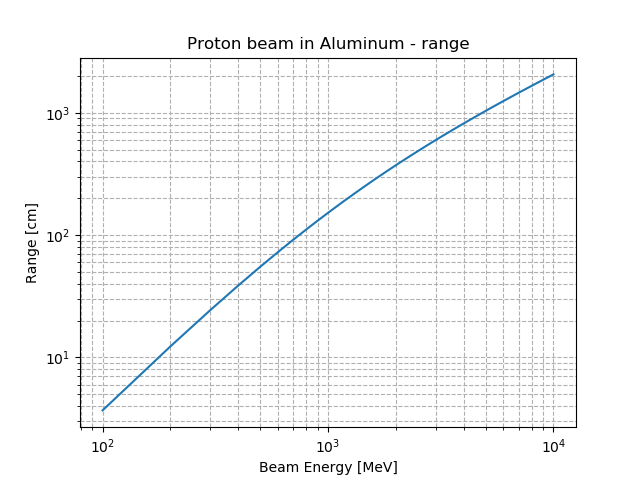
\includegraphics[width=0.7\textwidth]{Aluminumrange.png}
\caption{Range for proton beam in aluminum}
\label{fig:range}
\end{figure}

\item[d)] To compute the (average) distance traveled by a $10\si{\mega\electronvolt}$ escaping from the absorber it is sufficient to repeat the last calculation using as absorber material air. As usual the physical properties of air are from NIST, for $A$ and $Z$ the values are averaged on the main components according to NIST. The result is
\begin{align*}
d = 1.16\si{\metre}.
\end{align*}
To have a comparison, a same energy electron in Aluminum would be stopped after $6.1\si{\centi\metre}$, in agreement with the much lower density of air, that drastically reduces the number of collisions.

\end{itemize}

\end{enumerate}
%-----------------------------------------

\section*{Problem 3: Neutral particle interaction}
\begin{enumerate}
\item[a)] The probability $dP$ for a particle to interact when traveling thorugh a region $dx$ is proportional to the trajectory itself through the total reaction cross section $\sigma$ and the volume concentration $N$ of reaction centers:
\begin{align*}
dP = N\sigma dx
\end{align*}
Note that the total cross section $\sigma$ is a sum of various contributions.\\
By definign $\mathscr{P}(x)$ as the probability of having interacted after a distance $x$, we can regard $d\mathscr{P}$ -the probability of interacting in the region $dx$ - as the probability of not interacting in the region before $[1-\mathscr{P}(x)]$ times the probability $dP$ of interacting in the region $dx$ itself:
\begin{align*}
d\mathscr{P} = [1-\mathscr{P}(x)]\,N\sigma\,dx
\end{align*}
In terms of ODE:
\begin{align*}
\frac{d\mathscr{P}}{dx} = [1-\mathscr{P}(x)]\,N\sigma
\end{align*}
Through the substitution $\frac{d\mathscr{P}}{dx}=-\frac{d[1-\mathscr{P}]}{dx}$ and having defined the linear attenuation coefficient $\mu:=N\sigma$, the probability $P(x)$ of interaction after a distance $x$ is
\begin{align*}
P(x) = N\sigma\,[1-\mathscr{P}(x)] = N\sigma\,e^{-\mu x}.
\end{align*}
The intensity $I(x)$ is then just proportional to the interaction probability $P(x)$, with imposing the boundary condition $I(0)=I_o$:
\begin{align*}
I(x) = I_o\,e^{-\mu x}.\qquad\square
\end{align*}

\item[b)] To have attenuation of $1/e$ in the through lead it is enough to require the thickness $x$ to be
\begin{align*}
x = \mu_{Pb}(600\si{\kilo\electronvolt})^{-1}
\end{align*}
where $\mu_{Pb}(600\si{\kilo\electronvolt})$ is the attenuation coefficient, obtained from the mass attenuation coefficient at $600\si{\kilo\electronvolt}$\footnote{https://physics.nist.gov/PhysRefData/XrayMassCoef/ElemTab/z82.html}:
\begin{align*}
\mu_{Pb}(600\si{\kilo\electronvolt}) = \bigg(\frac{\mu}{\rho}\bigg)\bigg|_{600\si{\kilo\electronvolt}}\rho = 1.248\times10^{-1}\frac{\si{\square\centi\meter}}{\si{\gram}}\,11.35\frac{\si{\gram}}{\si{\cubic\centi\meter}}
\end{align*}
Therefore the thickness of the lead block needs to be
\begin{align*}
x =  0.71\si{\centi\meter}
\end{align*}

\item[c)] It is common to distinguish between 'high-energy' ($\gtrsim1\gev$), 'fast' ($\sim 0.1 - 10 \mev$) and 'slow' ($\lesssim \si{\electronvolt}$) neutrons, since the cross sections differ significantly for these energy thresholds. \\
High enery neutrons mostly undergo nuclear reactions causing target nuclei to fission in highly unstable fragments that decay afterwards. If the target nuclei are heavy, they will expel excess neutrons from the fragments ("spallation"). The collision between high energy neutrons and taget nucleons can also give rise to hadron production (mostly light pions, also heavier hadrons at higher energies).\\
For fast neutrons there is a strong energy dependence for the neutron-nucleon cross section and resonances are quite frequent. The most common process is neutron-nucleus elastic scattering, but there can also be inelastic scattering processes, leaving the nucleus in an excited state undergoing decay, as well as neutron capture, where the nucleus absorbs the incoming neutron and reaches stability through gamma decay, emission of charged particles or fission.\\
Slow neutrons mostly interact with elastic scattering and neutron capture until they reach thermal energy $\sim\frac{3}{2}k_bT$ and remain trapped inside the material.

  

\end{enumerate}
%-----------------------------------------

\section*{Problem 4:}
\begin{enumerate}
\item[a)] A cross section for a reaction can be defined simply as the transverse surface with respect to the beam/incoming particle flux inside which the reaction will happen. It is usually measured in $\si{barn}$ $(=10^{-24}\si{\square\centi\meter})$ 

\item[b)] Cherenkov effect is basically the emission of optical photons when a charged particle in a medium travels faster than light in the medium itself. 
A charged particle in the medium will cause a local electromagnetic perturbation that propagates isotropically as a spherical wave with velocity $v=\frac{c}{n}$, $n$ being the refraction index of the medium. If the velocity of the particle is greater than $\frac{c}{n}$, the wavefronts of the perturbations will not randomly dissolve as it would happen for a slower particle but they will add up in constructive interference on a plane that propagates with optical frequencies at n angle $\theta_C = \arccos(\frac{c}{n\,v})$ with respect to the charged particle trajectory.

\item[c)] Bremsstrahlung is the radiation emitted from an accelerating charged particle as predicted by the Larmor-Liénard formula
\begin{align*}
P = \frac{\mu_o q^2 \gamma^6}{6\pi c}\bigg( a^2 - \bigg|\frac{ \mathbf{v}\times\mathbf{a}}{c} \bigg|^2 \bigg)
\end{align*} 
where $P$ is the power of the emitted radiation, $q$ the charge of the particle, $\gamma$ the relativistic parameter, $\mathbf{a}$ the acceleration that the particle undergoes and $\mathbf{v}$ its velocity.\\
This means that any decelerating charged particle, i.e. hitting a target or being bent by a magnetic field, will emit electromagnetic radiation, and the effect will be more significant the higher the energy of the particle.
\end{enumerate}
%-----------------------------------------

\section*{Problem 5: Compton scattering}
\begin{enumerate}
\item[a)] Consider the frame where the photon is hitting the electron at rest. A sketch of the process is given in figure \ref{fig:compton}. The initial energy of the photon is $E_o$ (momentum $\frac{E_o}{c}$), while the final momentum of the electron is $p_e$ and for the photon $\frac{E}{c}$. $m$ is the electron mass.

\begin{figure}[!ht]
\centering
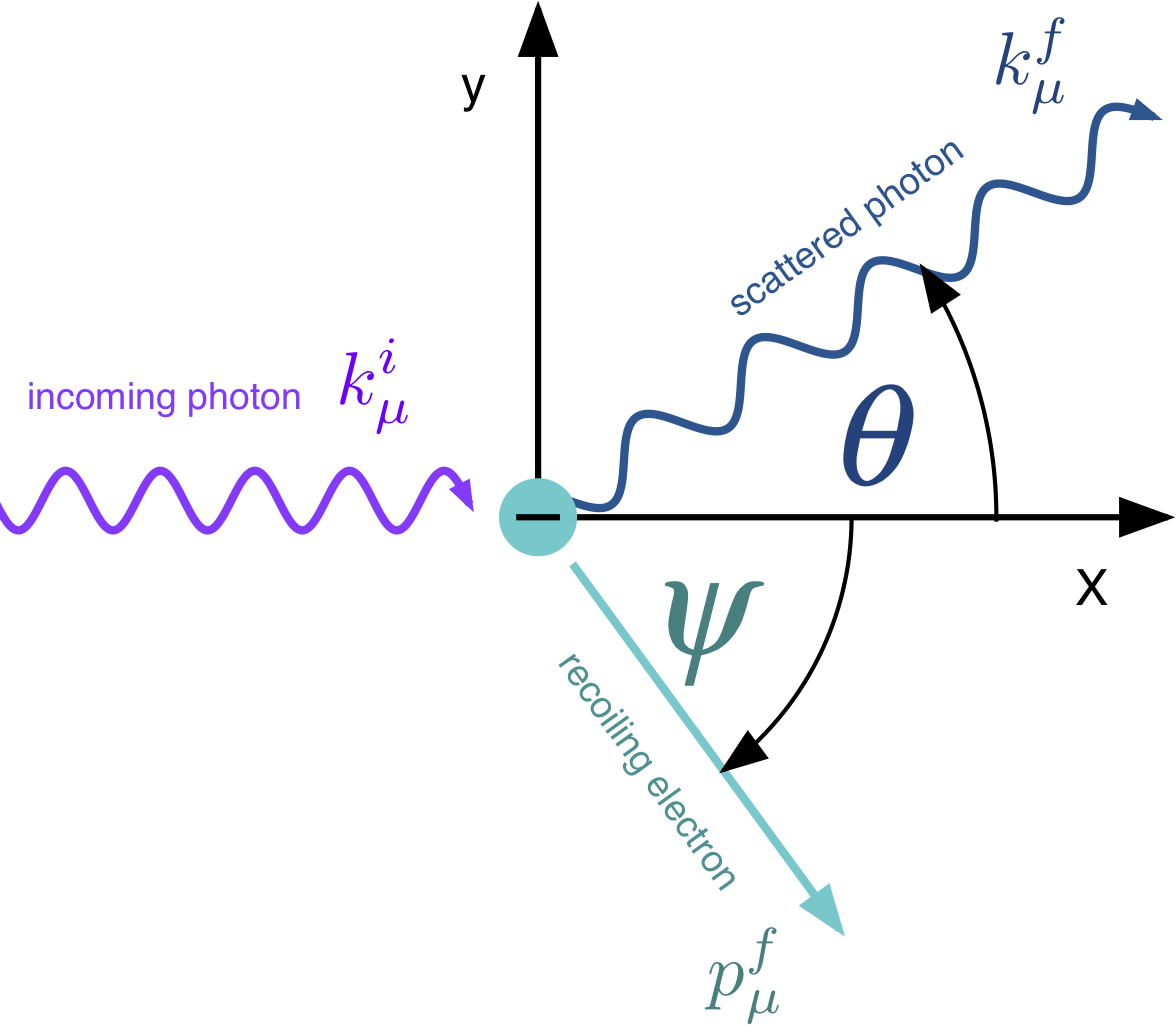
\includegraphics[width=0.45\textwidth]{Compton.png}
\caption{Compton scattering - scheme}
\label{fig:compton}
\end{figure}

Imposing momentum conservation in $x$ and $y$ direction result in
\begin{align*}
&\frac{E}{c}\sin\theta = p_e\sin\psi,\qquad\Rightarrow\qquad\sin\psi=\frac{E}{p_e\,c}sin\theta\\
&\frac{E_o}{c} = \frac{E}{c}\cos\theta + p_e\underbrace{\cos\psi}_{\sqrt{1-\sin^2\psi}} = \frac{E}{c}\cos\theta + p_e\sqrt{1-\bigg( \frac{E}{p_e\,c}\sin\theta \bigg)^2}
\end{align*}
the latter giving the expression
\begin{align}
\label{useful}
p_e^2c^2 = E_o^2+E^2-2E_oE\cos\theta.
\end{align}
Energy conservation then implies
\begin{align*}
E_o + mc^2 = E+\sqrt{m^2c^4+p_e^2c^2}
\end{align*}
that when substituting the expression for (\ref{useful}) and solving for E becomes
\begin{align}
\label{eq:comptonenergy}
E = \frac{1}{\frac{1-cos\theta}{mc^2}+\frac{1}{E_o}}.
\end{align}
By applying Planck's definition for photon energy $E_o=h\frac{c}{\lambda},\,E=h\frac{c}{\lambda'}$ and taking the inverse of the latter expression we get
\begin{align*}
\frac{\lambda'}{h\,c} = \frac{1-\cos\theta}{m\,c^2}+\frac{\lambda}{h\,c}\quad\Rightarrow\quad \lambda' - \lambda = \frac{h}{mc}\big( 1-\cos\theta \big)\quad\square
\end{align*}

\item[b)] The energy of a $1\mev$ photon after a $30\si{\degree}$ and $90\si{\degree}$ scattering can be easily found by applying the derived relation. Being $\cos(\pi/2)=1$ a $90\si{\degree}$ scattering will not result in energy loss since $\Delta E = h\,c\big( \frac{\lambda-\lambda'}{\lambda\lambda'}\big) = 0$.\\
 For the $30\si{\degree}$ scattering we have
\begin{align*}
&\lambda'-\lambda = \frac{h}{mc}\big( 1-\frac{\sqrt{3}}{2}\big) = 0.134\frac{h}{mc}\\
&\Rightarrow \lambda' = 0.134\frac{hc}{0.511\mev} + \frac{hc}{1\mev} =1.262\,\frac{hc}{\mev}\\
&\Rightarrow E = \frac{hc}{\lambda'} = 0.792\mev\qquad\square
\end{align*}

\item[c)] The latter calculation has been implemented in a few lines of code. To get the total energy deposited is necessary to calculate the photon energy after the first collision $E_1$ and use that value as input for the second collision to get the final energy after two collisions $E_2$. Then the energy deposited in the material $\Delta E$ is just the difference between the initial energy and the value after the second collision. Results are displayed in table \ref{tab:compton}.
\begin{table}[!ht]
\centering
\begin{tabular}{ccc}
\toprule
  $E_1$ & $E_2$ & $\Delta E$ \\
  \midrule
  $1.31\mev$ & $0.68\mev$ & $1.32\mev$ \\
  \bottomrule
\end{tabular}
\caption{Energy after first and second collision and energy distribution for $30\si{\degree}$ and $60\si{\degree}$ consecutive scattering}
\label{tab:compton}
\end{table}

\item[d)]The maximum energy deposition in a material is for backward scattering, i.e. $\theta = \pi$, that minimizes the final energy $E$ in equation \ref{eq:comptonenergy}.

The backward scatter energies can be found by calculating equation \ref{eq:comptonenergy} for $\theta = \pi$, while the energy deposition is just the difference between $E$ and the incoming energy $E_o$. Results are in table \ref{tab:edges}

\begin{table}[!ht]
\centering
\begin{tabular}{ccc}
\toprule
  $E_o$ & $E$ & Energy deposition \\
  \midrule
  $0.06\mev$ & $0.011\mev$ & $0.04\mev$ \\
  $1.332\mev$ & $1.12\mev$ & $0.21\mev$ \\
  $2.164\mev$ & $1.93\mev$ & $0.23\mev$ \\
  \bottomrule
\end{tabular}
\caption{Compton edges and backward scattered energies for different incoming photon energies}
\label{tab:edges}
\end{table}
\end{enumerate}

\pagebreak
%-----------------------------------------


\begin{thebibliography}{5}
\bibitem{Tavernier}S.Tavernier, \textit{Experimental techniques in Nuclear and Particle Physics}, Springer, 2010

\bibitem{Leo} W. R. Leo, \textit{Techniques for Nuclear and Particle Physics}, Springer-Verlag, 1987

\bibitem{Griffith} D. J. Griffiths, \textit{Introduction to electrodynamics}, Pearson, 2013

\end{thebibliography}
\end{document}